\documentclass[tikz,border=2pt]{standalone}
\usepackage[T1]{fontenc}
\usepackage{helvet}
\usepackage{amsmath}
\usetikzlibrary{arrows.meta,calc,positioning}
\renewcommand{\familydefault}{\sfdefault}
\definecolor{ink}{HTML}{202124}
\definecolor{teal}{HTML}{167C72}
\definecolor{tealfill}{HTML}{DDEEE9}
\definecolor{orange}{HTML}{D97706}
\definecolor{muted}{HTML}{70757A}
\tikzset{
  card/.style={draw=ink!65,line width=.55pt,rounded corners=2pt,fill=white},
  cardfocus/.style={card,draw=teal,line width=.9pt,fill=tealfill!45},
  arrow/.style={-{Stealth[length=2mm]},draw=teal,line width=.75pt},
  title/.style={font=\sffamily\bfseries\fontsize{11}{13}\selectfont,text=ink,align=center},
  body/.style={font=\sffamily\fontsize{8.2}{9.8}\selectfont,text=ink,align=center},
  small/.style={font=\sffamily\fontsize{7}{8.5}\selectfont,text=muted,align=center},
  edgeLabel/.style={font=\sffamily\bfseries\fontsize{7.5}{9}\selectfont,text=ink,align=center,fill=white,inner sep=1.5pt},
  question/.style={font=\sffamily\itshape\fontsize{7}{8.5}\selectfont,text=muted,align=center}
}
\begin{document}
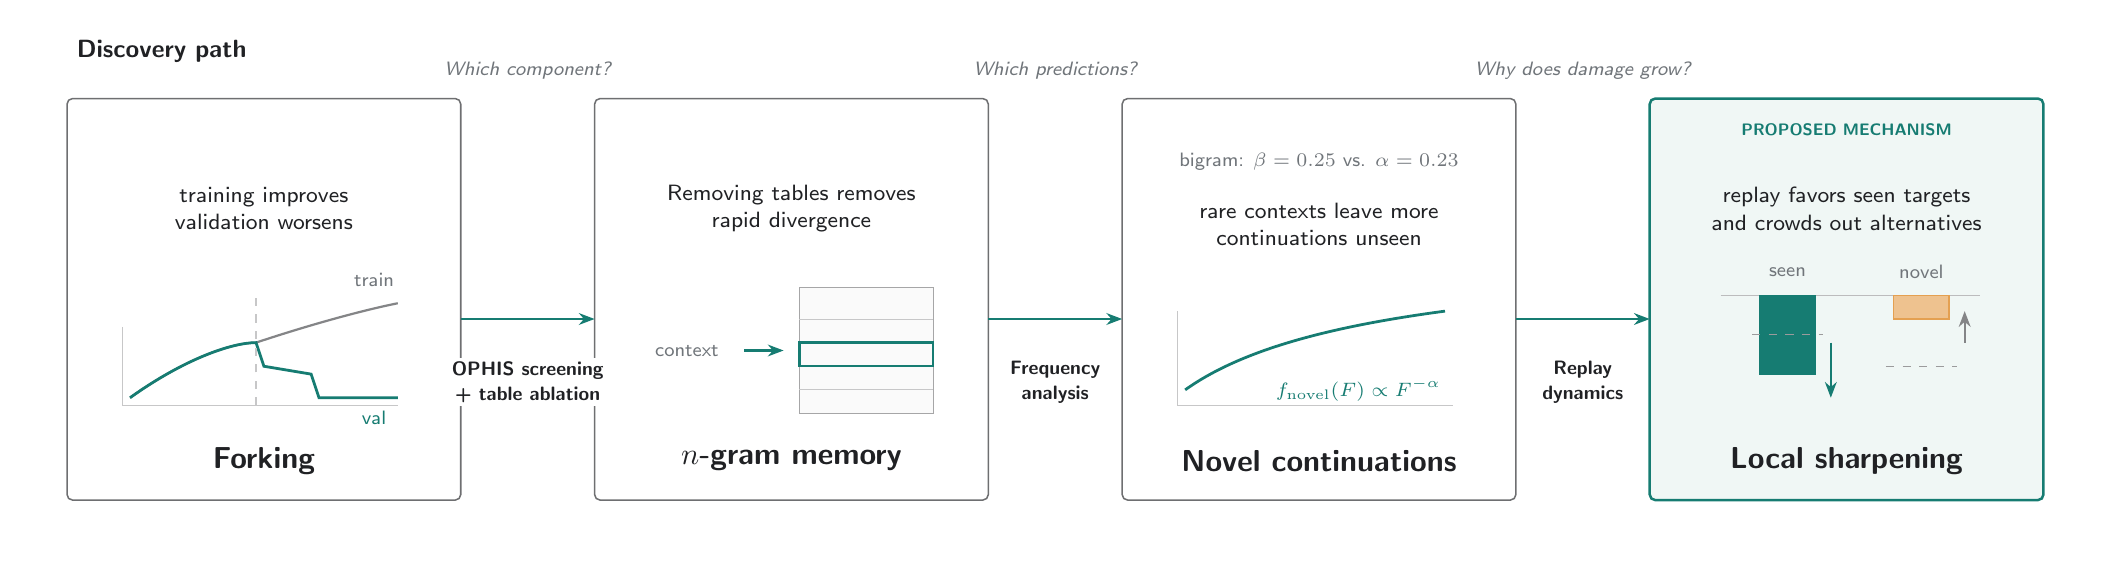
\begin{tikzpicture}[x=1mm,y=1mm]
\path[use as bounding box] (0,0) rectangle (260,65);
\node[font=\sffamily\bfseries\fontsize{9}{11}\selectfont,text=ink,anchor=west] at (5,62) {Discovery path};
\draw[card] (5,5) rectangle (55,56);
\draw[card] (72,5) rectangle (122,56);
\draw[card] (139,5) rectangle (189,56);
\draw[cardfocus] (206,5) rectangle (256,56);
\node[title] at (30,10) {Forking};
\node[title] at (97,10) {$n$-gram memory};
\node[title] at (164,10) {Novel continuations};
\node[title] at (231,10) {Local sharpening};
\draw[ink!25,line width=.35pt] (12,27) -- (12,17) -- (47,17);
\draw[ink!55,line width=.8pt] (13,18) .. controls (20,23) and (26,25) .. (29,25) .. controls (35,27) and (42,29) .. (47,30);
\draw[teal,line width=1pt] (13,18) .. controls (20,23) and (26,25) .. (29,25) -- (30,22) -- (36,21) -- (37,18) -- (47,18);
\draw[ink!25,dashed,line width=.4pt] (29,17)--(29,31);
\node[small,text=teal] at (44,15.5) {val};
\node[small] at (44,33) {train};
\node[body] at (30,42) {training improves\\validation worsens};
\node[small,anchor=east] at (89,24) {context};
\draw[arrow] (91,24)--(96,24);
\draw[draw=ink!40,fill=black!2] (98,16) rectangle (115,32);
\foreach \y in {19,22,25,28}{\draw[ink!25,line width=.3pt] (98,\y)--(115,\y);}
\draw[teal,line width=.9pt] (98,22) rectangle (115,25);
\node[body] at (97,42) {Removing tables removes\\rapid divergence};
\draw[ink!25,line width=.35pt] (146,29) -- (146,17) -- (181,17);
\draw[teal,line width=1pt] (147,19) .. controls (154,24) and (165,27) .. (180,29);
\node[small,text=teal] at (169,19) {$f_{\rm novel}(F)\propto F^{-\alpha}$};
\node[body] at (164,40) {rare contexts leave more\\continuations unseen};
\node[small] at (164,48) {bigram: $\beta=0.25$ vs. $\alpha=0.23$};
\draw[ink!30,line width=.35pt] (215,31)--(248,31);
\draw[teal,fill=teal] (220,21) rectangle (227,31);
\draw[orange!70,fill=orange!45] (237,28) rectangle (244,31);
\draw[ink!45,dashed,line width=.45pt] (219,26)--(228,26);
\draw[ink!45,dashed,line width=.45pt] (236,22)--(245,22);
\draw[arrow] (229,25)--(229,18);
\draw[arrow,draw=ink!55] (246,25)--(246,29);
\node[small] at (223.5,34) {seen};
\node[small] at (240.5,34) {novel};
\node[body] at (231,42) {replay favors seen targets\\and crowds out alternatives};
\node[font=\sffamily\bfseries\fontsize{6.5}{8}\selectfont,text=teal] at (231,52) {PROPOSED MECHANISM};
\draw[arrow] (55,28)--(72,28);
\draw[arrow] (122,28)--(139,28);
\draw[arrow] (189,28)--(206,28);
\node[edgeLabel] at (63.5,20) {OPHIS screening\\+ table ablation};
\node[edgeLabel] at (130.5,20) {Frequency\\analysis};
\node[edgeLabel] at (197.5,20) {Replay\\dynamics};
\node[question] at (63.5,59.5) {Which component?};
\node[question] at (130.5,59.5) {Which predictions?};
\node[question] at (197.5,59.5) {Why does damage grow?};
\end{tikzpicture}
\end{document}
